\chapter{Concepts}
Pour parvenir à créer une machine capable de trier des billes de roulement à bille, il nous a fallu résoudre deux problèmes: l'acheminement des billes, et leur tri.

%\section{Répartition du projet}

Vu que nous étions un groupe de quatre étudiants, nous avons décidé de répartir la machine en quatre parties. Les deux problèmes principaux susmentionnés fûrent les deux divisés en deux. Ensuite, chacun de nous s'occupait de concevoir le/les mécanisme/s nécessaires pour que la machine comme ensemble puisse satisfaire les conditions imposées par le cahier des charges. Notre division fut la suivante:
\begin{itemize}
    \item Réservoir pour les billes mixtes
    \item Acheminement
    \item Séparation \& tri
    \item Réservoirs pour les billes triées
\end{itemize}

\section{Réservoir pour billes mixtes}

\subsection{Concepts imaginés}
\begin{itemize}
    \item Nous avons dans un premier temps imaginé un réservoir rectangulaire, en forme de parallélépipède creux. Mais l’usinage d’une telle pièce exige le forage d’un cube de métal, ce qui entraîne un important gaspillage. 
    \item Ainsi, nous avons pensé à assembler des plaques ensemble grâce à des vis, afin d’économiser de la matière et de diminuer le coût de notre machine. L'inconvénient était alors le grand nombre de pièces nécessaires pour un simple réservoir (parois, vis). 
    \item Finalement, l’idée d’un cylindre creux associé à un fond sphérique s’est imposée comme étant la plus économe et la plus rapide à assembler. En effet, le cylindre peut être un simple tuyau coupé à la bonne longueur et usiné sur un seul côté pour permettre la sortie du réservoir. Le fond incliné consiste en une plaque sphérique usinée pour obtenir l'inclinaison nécessaire à l'évacuation des billes. De plus, les deux pièces peuvent facilement être assemblées grâce à 2 vis.
\end{itemize}

%image manque

\section{Acheminement}
Ce mécanisme devait satisfaire plusieurs contraintes et demandes à la fois. Il était préscrit que notre machine s'opère à une main et que le tri des billes soit déclenché par l'utilisateur et ne se déclenche pas soi-même. En plus, tout coincement devait être prévenu.

Les options élaborés en groupe étaient alors les suivantes:\\
Pour l'entraînement des billes:

\subsection{Convoyeur à vis}
Notre première idée fut une convoyeur à vis qui transporte les billes vers les railles. Les billes sortent alors du réservoir mixte et roulent vers la convoyeur à vis. Là ils tombent dedans et la rotation provenant de la manivelle les entraîne vers les rails.

%image manque

Mais après tout cette idée fut impraticable à cause de plusieurs raisons. Premièrement le coût est sûrement plus élevé que celui des autres alternatives. Et deuxièmement on ne trouvait pas de solution satisfaisante pour empêcher le coincement des billes.

\subsection{Cylindre avec des trous}
La deuxième option qu'on a élaboré était un cylindre long avec des petits trous dedans. Comme avec la convoyeur à vis les billes roulent hors du réservoir mixte et tombent dans les trous du cylindre tournant. Comme pour la première idée on prévoyait une manivelle pour l'opération du mécanisme.

%image manque

Cette option était finalement abandonnée car la fabrication aurait coûté plus chère que celle de la troisième option (cf. en bas). On aurait du faire des alésages très précis au lieu de juste fraiser des roues dentées.

\subsection{Roues dentées décalés}
Notre troisième idée était de simplement monter des roues dentées sur une barre et de les décaler d'un dent à la fois.
%image manque

Les billes provenant du réservoir mixte roulent alors doucement (à cause de la pente modérée)  vers les roues dentés. Après ils tombent entre les dents et sont entraînés vers les railles par la rotations induite par l'opération de la manivelle.

%image de l'ensemble manque

Pour le déblocage:
\subsection{Un pivot positionné à la sortie du réservoir pour empêcher l'empilement des billes} 
Notre première option pour le déblocage fût un pivot positionné à la sortie du réservoir mixte. Ce pivot aurait été connecté à l'axe de rotation de l'acheminement par une chaîne ou une autre connexion permettant la transformation de la rotation en "pivotement". Ainsi tout empilement néfaste des billes dans le réservoir aurait été empêche par l'utilisation de la manivelle.

%image manque

\subsection{Couvercle pour la roue dentée}
Plutôt comme mécanisme de déblocage supplémentaire on prévoyait un couvercle pour le mécanisme d'acheminement. Avec des dents/trous d'une profondeur de 5 mm même les billes de diamètre 7 pourront passer sous un couvercle à distance 2,5 mm du mécanisme d'acheminement. Par contre dès qu'il y aura deux billes dans un/e dent/trou même pour le pire des cas (deux billes de la taille la plus petite) la deuxième bille heurtera le couvercle en dessous ou exactement avec son centre de masse. Ainsi elle sera enlevée et on aura l'assurance qu'à chaque fois un a qu'une bille par dent/trou.

% mettre plusieurs images

\section{Séparation \& tri (rails)}

\subsection{Séparation}
Après que les billes sont acheminés hors du réservoir, les billes doivent être séparées de manière successive pour ne pas bloquer le mécanisme de tri que suit.

\subsubsection{Coins}
La première idée était de ordonner les billes en utilisant des coins sur un plan inclinée. Cette méthode menait à plusieurs problèmes: la pièce est devenue très compliqué à fabriquer, cause des composantes arrondies et le risque du coincement des billes ne pourrait pas être éliminé suffisamment.

% image

\subsubsection{Rainures}
Après avoir abandonné l'idée avec les coins, nous avons cherché une autre solution pour guider les billes qui arrivent de la roue dentée sur les rails. Notre deuxième option était de séparer les billes, pas avec des autres pièces, mais par leur propre poids. Cette idée consistait d'une plaque avec des rainures en forme arrondi ou linéaire. Ces deux options sont pas optimales non plus, il fallait fraiser les cercles ou les formes "V" dans une plaque, un défaut que augmentera le coût de cette pièce beaucoup plus.

% image

\subsection{Tri}
À ce point vient la partie principale de tout l'ensemble, le tri des billes en dépendance de leur diamètre.

\subsubsection{Ecartement graduel}
Notre première idée pour trier les billes en trois différentes tailles, était d'utiliser des rails quasi-perpendiculaires qui s'écartaient de manière graduelle. 

% image

\subsubsection{Ecartement séquentiel}
Pour résoudre les faiblesses de l'écartement graduel, nous l'avons adapté et sont arrivés au écartement séquentiel. L'avantage de cette technique est que les billes ne ralentissent pas dans leur rails, mais roulent avec une vitesse constante, jusqu'au point où se trouve le saut d'un diamètre au prochain et tombent dans le réservoir au-dessous.

% image

\subsubsection{Plaque inclinée et barres}
Une idée alternative aux solutions avec les rails, était de monter des barres au-dessus d'une plaque inclinée de manière que les billes avec un diamètre donné seront transportées à coté de la plaque et les billes plus petites passaient au-dessous de la barre jusqu'à la prochaine.

% image

\subsubsection{Ecartement séquentiel avec rainures}
L'idée finale qui était incorporée dans le projet, est celle des rails avec un écartement séquentiel en combinaison avec les rainures en forme "V" tous dans une seule pièce. Comme ça, les parties de la séparation des billes et leur tri en combiné et la complexité de l'ensemble et réduite même plus.

\section{Réservoir pour les billes triées}
Les exigences au réservoir pour les billes triées sont clairs: Il nous fallait trois containers placés ainsi que tous les billes d'une même taille tombent dans le réservoir prévu pour leur taille.

\subsection{Premier brouillon}
La construction des rails nous a donné un espace limité ou les billes d'une taille tombent. Ca veut dire qu'il y a trois rectangles l'un juste à côte de l'autre. Pour simplifier la construction nous les avons choisi de la même taille, indépendant de la taille des billes. Le premier brouillon était donc un réservoir avec un fond incliné pour que les billes s'accumulent tous de la même côté.

\begin{figure}
    \centering
    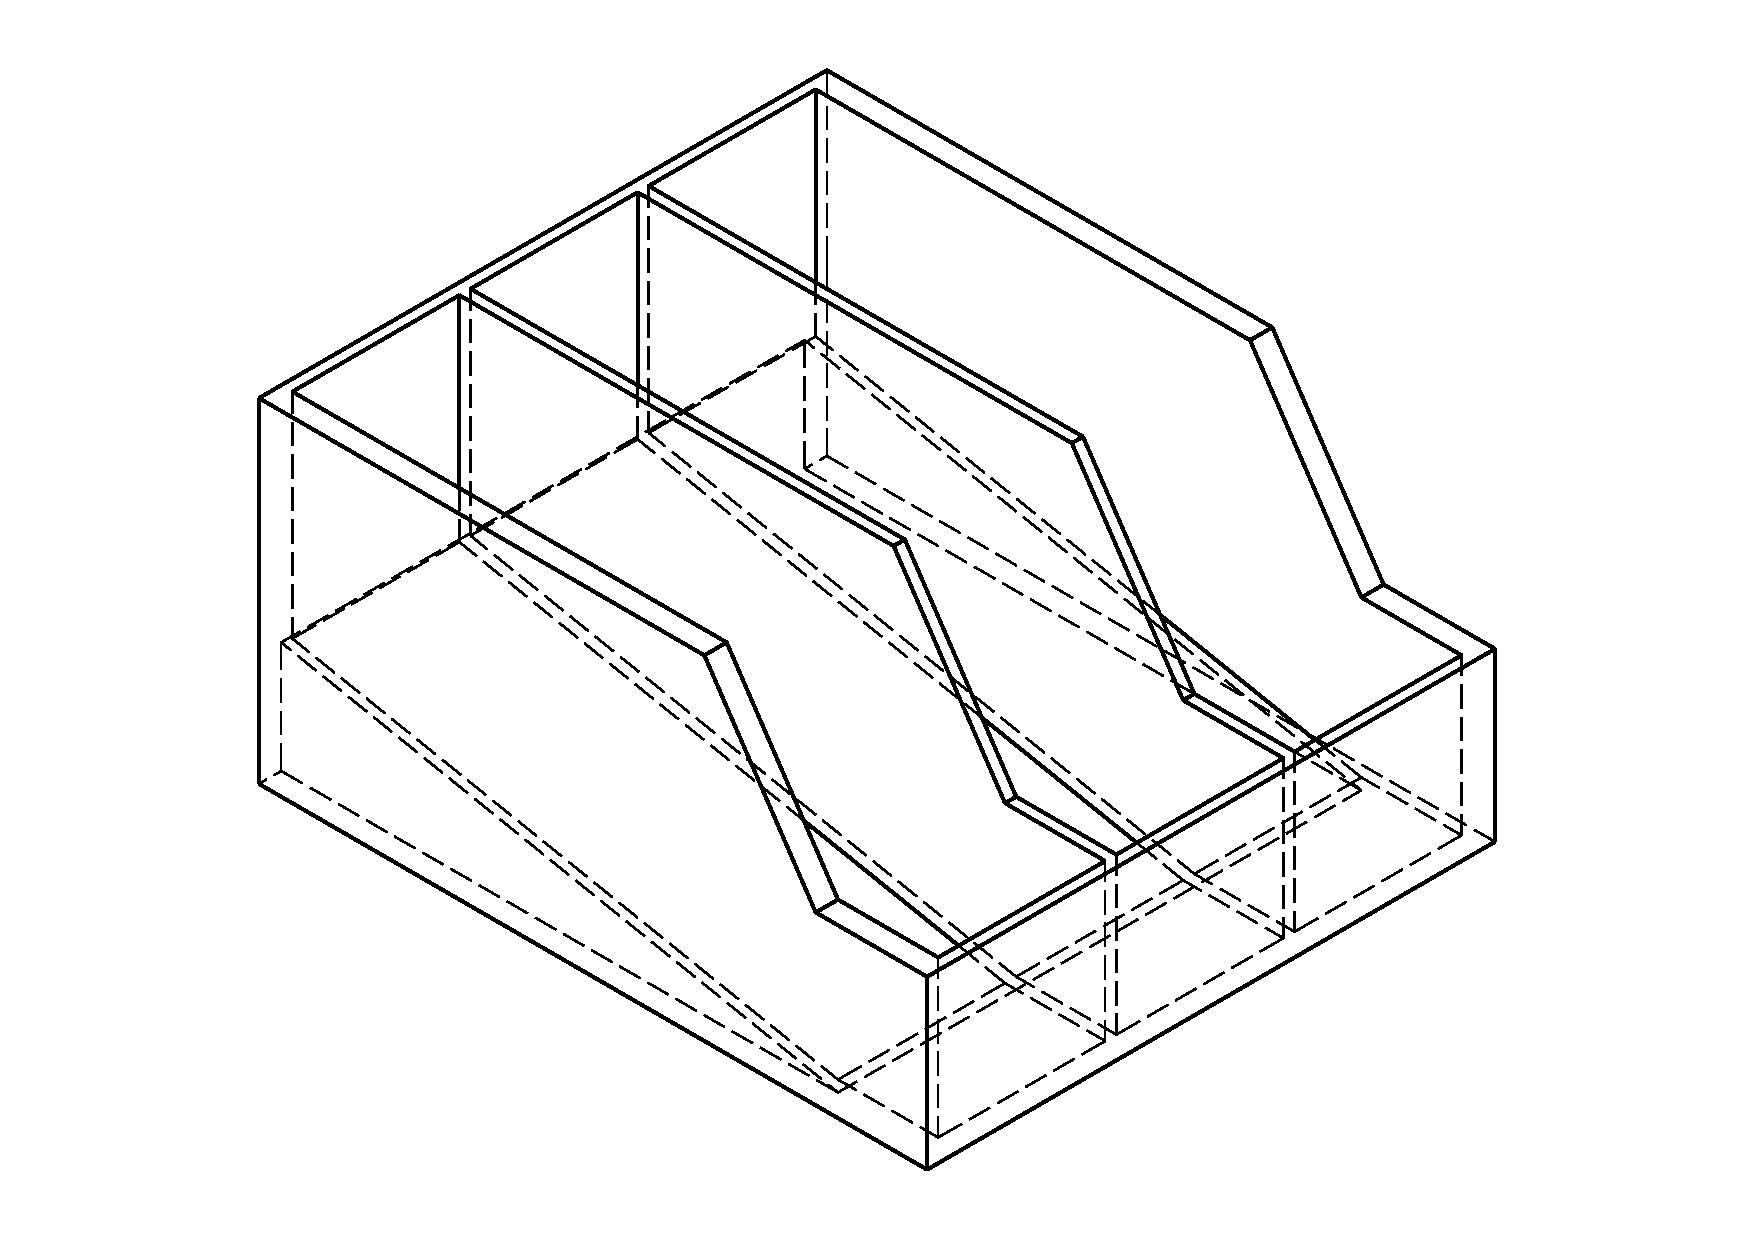
\includegraphics[width=\textwidth]{Graphics/Reservoir_final/PREMIER_BROUILLON.pdf}
    \caption{Premier brouillon}
    %\label{fig:B1}
\end{figure}

Les billes devaient ainsi être enlevé par main du réservoir qui peut poser des problèmes à cause de la petite taille. Nous avons alors décidé de faire des containers qui peuvent être enlevé lors de la prise des billes. 

\subsection{Deuxième brouillon}
La forme choisie pour les containers était un cube. Alors il nous fallait une rampe afin de canaliser les billes dans les cubes.  Le dimensionnement des cubes se déroulait en prise en compte de la taille des billes. Au pire cas les 300 billes sont de la même taille. Alors les cubes doivent être capable de prendre 300 billes de la taille respective. Pour simplifier la construction les cubes ont tous la même taille sans respecter la taille des billes. Le volume des cubes à alors été donné par:
\begin{equation}
    V = 7^3\ 300\ d \approx 7^3\ 300\ 0.75 = 77'175\ mm^3
    \label{eq:volumereservoirfin}
\end{equation}

Où \(d = \frac{ \pi }{3\sqrt{2}} \approx 0.75\) est la densité volumique de l'empilement compact de billes. La longueur des arêtes intérieures du cube sont alors donné par: 
\[l\textsubscript{int}=\sqrt[3]{77'175\ mm^3} \approx 42.5\ mm\]

Avec une certaine tolérance si les billes ne s'empilent pas aussi compacte que possible, nous avons choisi une longueur d'arête extérieure de \({l\textsubscript{ext}=49~mm}\). Pour utiliser le place de la manière la plus efficace, nous avons inversé l'orientation de la rampe au milieu. Comme ça les containers ne se trouvent pas tous sur une ligne, ce qui rends la machine plus compacte. 

\begin{figure}
    \centering
    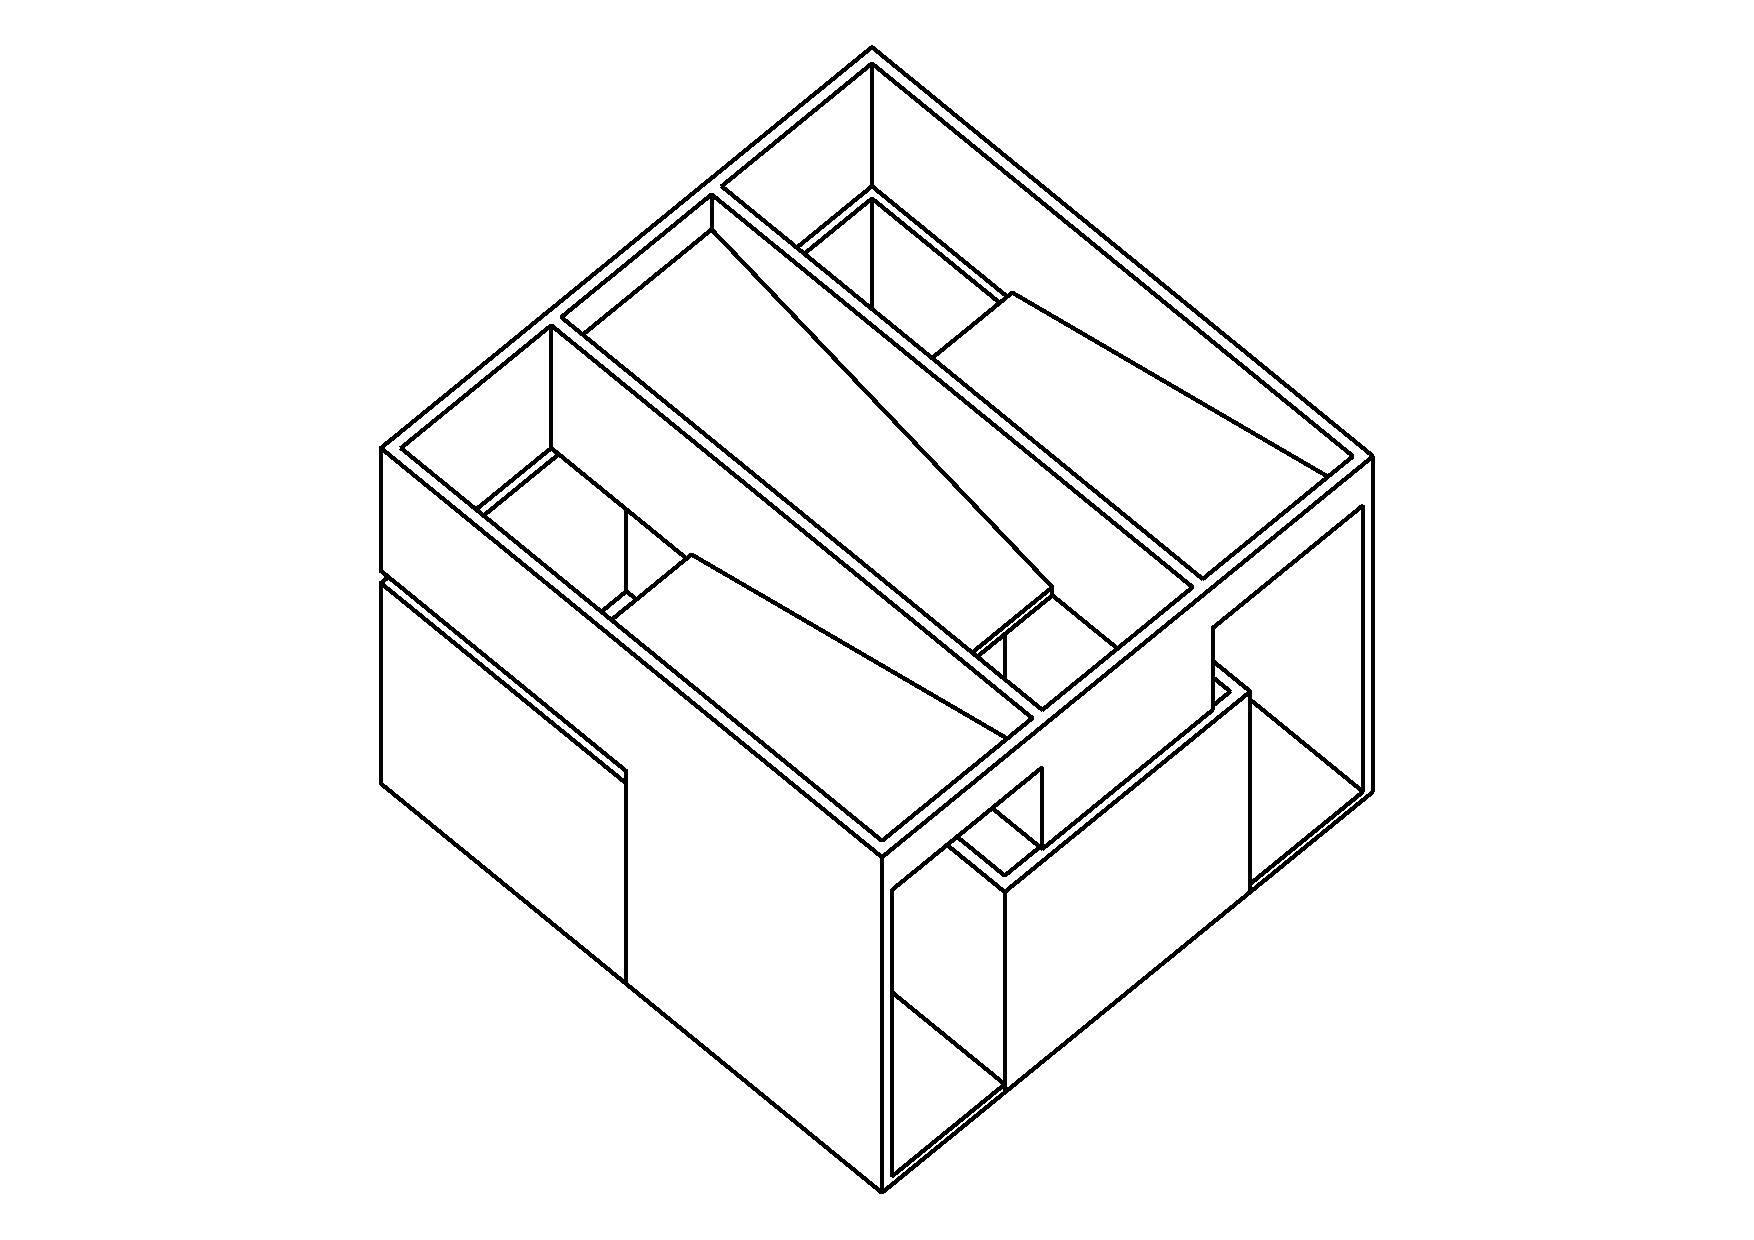
\includegraphics[width=\textwidth]{Graphics/Reservoir_final/DEUXIEME_BROUILLON.pdf}
    \caption{Deuxième brouillon}
    %\label{fig:B2}
\end{figure}


\subsection{Troisième brouillon}
Vue que l'assemblage avec vis de plus de 4 mm n'est pas possible pour certaines  éléments du deuxième brouillon (i.e. les cubes) et que la fabrication par fraisage à partir d'un seul bloc est bien trop coûteux et inefficace, nous avons remanié le brouillon en respectant ces aspects. La forme oblong des containers nous a permis de supprimer les rampes au dessous du réservoir et donc de diminuer le nombre d'éléments.

\begin{figure}
    \centering
    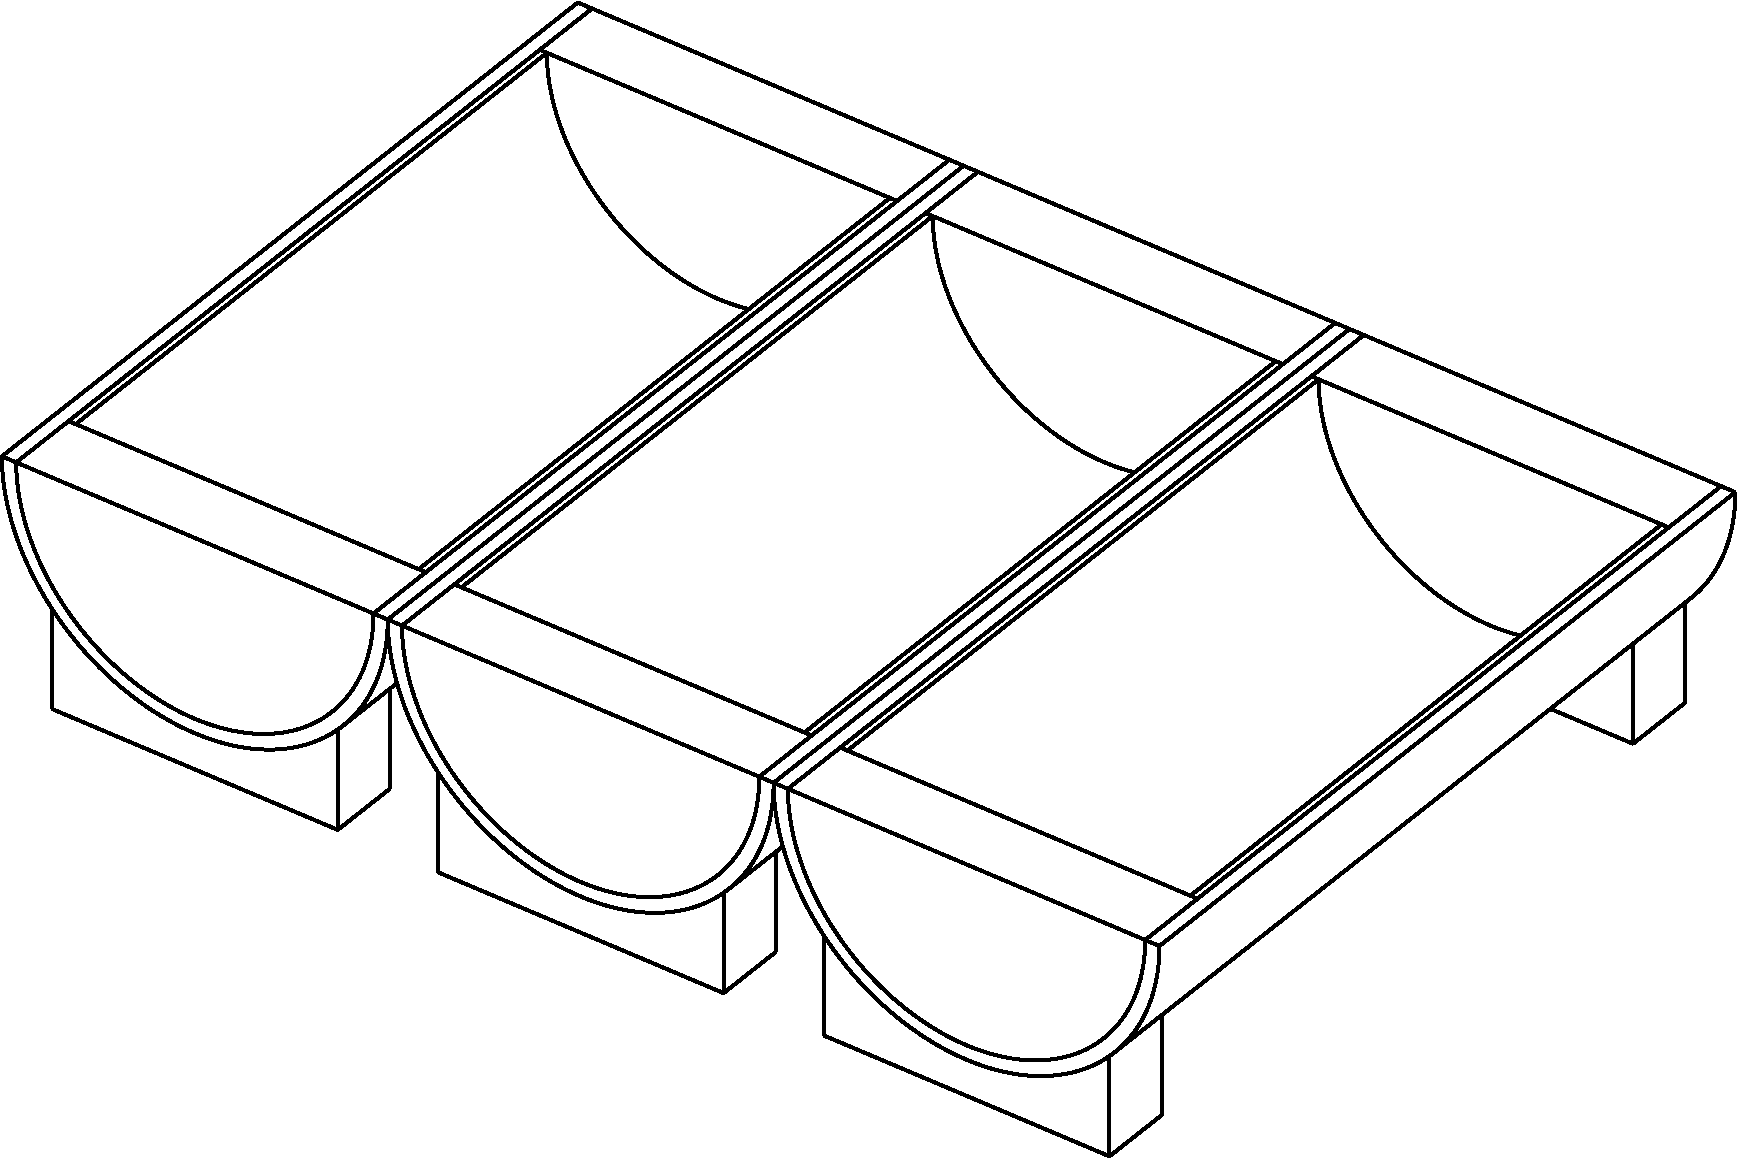
\includegraphics[width=\textwidth]{Graphics/Reservoir_final/TROISIEME_BROUILLON.pdf}
    \caption{Troisième brouillon}
    %\label{fig:B3}
\end{figure}

%\section{Acheminement}
%Pour l'acheminement des billes, nous avons tout d'abord imaginé un réservoir au fond incliné contenant les billes, et débouchant sur une série de roues dentées qui permettent de réguler le flux de billes.

%Ensuite, nous avons dû imaginé un mécanisme permettant d'acheminer les billes vers la zone de tri de manière régulée, tout en évitant absolument le coincement. Ainsi, l'idée de routes dentées dimensionnées pour contenir exactement une bille dans chaque compartiment s'est imposée comme étant la meilleure. En effet, une série de roues dentées décalées d'une dent (...) permet de prélever un nombre précis de billes en vue du tri.
%Les routes dentées sont actionnées grâce à une manivelle qui transmet le mouvement de rotation grâce à un arbre.

%\section{Tri}
%Pour le tri des billes, nous avons développé un système de rails parallèles, s'écartant par pallier. Cela permet de récolter les petites billes d'abord, les moyennes ensuite et finalement les plus grosses. L'écartement par pallier permet aussi d'éviter le coincement. En effet, nous avions tout d'abord pensé à un écartement progressif des rails, mais les billes ralentissent alors fortement avant de tomber, ce qui peut provoquer l'arrêt des billes suivantes. En effet, plus le diamètre de la bille se rapproche de la distance entre les rails, plus la bille descend, et son axe de rotation se rapproche de son axe de symétrie horizontal. Il en résulte une augmentation de la vitesse de rotation de la bille, et une diminution de sa vitesse horizontale. Ainsi, la bille qui suit risque de frotter contre celle qui ralentit, et la force de frottement entre les deux, amplifiée par l'augmentation de la vitesse angulaire de la première bille, risque de stopper les billes sur le rails, bloquant alors le mécanisme.